\documentclass[11pt,openany]{article}

\input{cryptanalysis-note-setup}
%Tikzpicture
\usepackage{graphicx}
\usepackage{tikz}
\usepackage{tikz-cd}
\usepackage{pgfplots}
\usetikzlibrary{shapes.geometric, calc}
\usetikzlibrary{angles, quotes}
\usetikzlibrary{arrows, arrows.meta}
\usetikzlibrary{patterns,patterns.meta}
\usetikzlibrary{positioning}
\usetikzlibrary{decorations.markings}
\usetikzlibrary{hobby}

%\input{../category-theory-setup-tcolorbox}
% Header and footer formatting

\pagestyle{fancy}
\fancyhead{}
\fancyhf{}
\rhead{\textcolor{TealBlue2}{\textbf{Cryptanalysis-FINAL}}}%\rule{3cm}{0.4pt}}
\lhead{\textcolor{TealBlue2}{\textbf{Lecture-FINAL}}}
% Define footer
\newcommand{\footer}[1]{
\begin{flushright}
	\vspace{2em}
	\includegraphics[width=2.5cm]{school_logo.jpg} \\
	\vspace{1em}
	\textcolor{TealBlue2}{\small\textbf{#1}}
\end{flushright}
}
%\rfoot{\large Department of Information Security, Cryptogrphy and Mathematics, Kookmin Uni.\includegraphics[height=1.5cm]{school_logo.jpg}}
\fancyfoot{}
\fancyfoot[C]{-\thepage-}

\input{cryptanalysis-note-thm}
%Tcolorbox
\usepackage[most]{tcolorbox}
\usepackage{varwidth}
\tcbset{colback=white, arc=5pt}

\newtcolorbox{defbox}[2][]{
	enhanced,
	colframe=defcolor, coltitle=white,
	title={\bf #2},#1
}

\newtcolorbox{probox}[2][]{
	enhanced,
	colframe=procolor, coltitle=white,
	title={\bf #2},#1
}


\newtcolorbox{thmbox}[2][]{
	enhanced,
	colframe=thmcolor, coltitle=white,
	title={\bf #2},#1
}

\newtcolorbox{corbox}[2][]{
	enhanced,
	colframe=corcolor, coltitle=white,
	title={\bf #2},#1
}
% Common

\newcommand{\N}{\mathbb{N}}
\newcommand{\Z}{\mathbb{Z}}
\newcommand{\Q}{\mathbb{Q}}
\newcommand{\R}{\mathbb{R}}
\newcommand{\C}{\mathbb{C}}
\newcommand{\F}{\mathbb{F}}

\newcommand{\ie}{\textnormal{i.e.}}
\newcommand{\sol}{\textcolor{magenta}{\bf Sol}}

\newcommand{\inv}[1]{#1^{-1}}
\newcommand{\of}[1]{\left( #1 \right)} 

\newcommand{\uniform}{\overset{\$}{\leftarrow}}
\newcommand{\from}{\leftarrow}

\newcommand{\zero}{\textcolor{red}{\texttt{0}}}
\newcommand{\one}{\textcolor{red}{\texttt{1}}}
\newcommand{\binaryfield}{\set{\zero,\one}}

% for Cryptanalysis

\newcommand{\id}{\textnormal{Id}}
\newcommand{\ddt}{\mathsf{DDT}}

% for Category Theory

\newcommand{\category}{\mathcal{C}}

\newcommand{\obj}[1]{\mathsf{obj}\left(#1\right)}
\newcommand{\homo}[1]{\mathsf{hom}\left(#1\right)}
\newcommand{\mor}[1]{\mathsf{mor}\left(#1\right)}


\newcommand{\dom}[1]{\mathsf{Dom}\left(#1\right)}
\newcommand{\cdm}[1]{\mathsf{Cdm}\left(#1\right)}

\newcommand{\op}{\textnormal{op}}

% for Lambda Calculus
\newcommand{\src}{\texttt{input}}
\newcommand{\target}{\texttt{output}}
\newcommand{\true}{\mathsf{T}}
\newcommand{\false}{\textsf{F}}
\usepackage{pifont}% http://ctan.org/pkg/pifont
\newcommand{\xmark}{\ding{55}}%

\setstretch{1.25}
\begin{document}
\pagenumbering{arabic}
\begin{center}
	\huge\textbf{Cryptanalysis - FINAL}\\
	\vspace{0.5em}
	\normalsize{\today}\\
	\vspace{0.5em}
	\large\textbf{Ji, Yong-hyeon}\\
	\vspace{0.5em}
\end{center}

\section{2021}
\begin{enumerate}[\bf 1.]
	\item 치환함수 $S:\set{0,1}^3\to\set{0,1}^3$가 다음과 같이 정의되었다고 하자.
	\begin{table}[h!]\centering\setstretch{1.5}
		\begin{tabular}{|c||c|c|c|c|c|c|c|c|}
			\hline
			$x$ & 0(000) & 1(001) & 2(010) & 3(011) & 4(100) & 5(101) & 6(110) & 7(111) \\
			\hline
			$S[x]$ & 0 & 2 & 4 & 6 & 5 & 7 & 3 & 1 \\
			\hline
		\end{tabular}
	\end{table}
	\begin{enumerate}[(a)]
		\item 입력차분이 $\alpha=4$일 때, 출력차분이 $\beta$가 될 확률 $P[\alpha\to\beta]$의 최댓값과 그 때의 $\beta$를 구하면?
		\item 입력 마스크가 $a=6(110)$이고 출력 마스크가 $b=2(010)$일 때 \[
		NS(a,b)=\set{x\mid a\cdot x=b\cdot S[x]}
		\]의 원소의 개수는? 임이의 입력 $x$에 대하여 $a\cdot x=b\cdot S[x]$가 만족될 확률은?
	\end{enumerate}
	\begin{proof}[\sol]
		\ \begin{enumerate}[(a)]
			\item 
			\ \begin{table}[h!]\centering\setstretch{1.25}
				\begin{tabular}{cc|cc|c}
					\toprule[1.2pt]
					$x$ & $x\oplus 100$ & $S[x]$ & $S[x\oplus 100]$ & $\beta=S[x]\oplus S[x\oplus 100]$\\ \hline
					000 & 100 & 000 & 101 & 101 \\
					001 & 101 & 010 & 111 & 101 \\
					010 & 110 & 100 & 011 & 111 \\
					011 & 111 & 110 & 001 & 111 \\
					100 & 000 & 101 & 000 & 101 \\
					101 & 001 & 111 & 010 & 101 \\
					110 & 010 & 011 & 100 & 111 \\
					111 & 011 & 001 & 110 & 111 \\
					\bottomrule[1.2pt]
				\end{tabular}
			\end{table}\\ 따라서 $\beta\in\set{(101)_2, (111)_2}=\set{5,7}$ 일 때, $$
			P[100\to 101]=\frac{1}{2}=P[100\to 111]$$ 이다.
			\newpage
			\item Let $x=(x_2x_1x_0)_2$ and $S[x]=(y_2y_1y_0)_2$. Consider $a=(110)_2$ and $b=(010)_2$: 
%			\begin{figure}[h!]\centering
%				\begin{tikzpicture}[>=Latex, node distance=1cm and 0cm]
%					% Nodes for inputs x
%					\node (x2) {\textcolor{red}{$x_2$}};
%					\node (x1) [right=of x2] {\textcolor{red}{$x_1$}};
%					\node (x0) [right=of x1] {$x_0$};
%					
%					% S-Box
%					\node (S) [draw, minimum size=1.5cm, below=of x1, xshift=0cm] {S};
%					
%					% Nodes for outputs y
%					\node (y2) [below=of S, xshift=-.5cm] {$y_2$};
%					\node (y1) [right=of y2] {\textcolor{red}{$y_1$}};
%					\node (y0) [right=of y1] {{$y_0$}};
%					
%					% Arrows from x to S
%					\draw[->, red, line width=1.25] (x2) -- (x2|-S.north);
%					\draw[->, red, line width=1.25] (x1) -- (x1|-S.north);
%					\draw[->] (x0) -- (x0|-S.north);
%					
%					% Arrows from S to y (ensuring alignment with x_i nodes)
%					\draw[->] (S.south-|x2) -- (x2|-y2.north);
%					\draw[->, red, line width=1.25] (S.south-|x1) -- (x1|-y1.north);
%					\draw[->] (S.south-|x0) -- (x0|-y0.north);
%				\end{tikzpicture}
%			\end{figure}\ \\	
			\begin{table}[h!]\centering\renewcommand{\arraystretch}{1}
				\begin{tabular}{ccc|ccc|cc}
					\toprule[1.2pt]
					\textcolor{red}{$[x_2]$} & \textcolor{red}{$[x_1]$} & $x_0$ & $y_2$ & \textcolor{red}{$[y_1]$} & {$y_0$} & $a\cdot x=b\cdot y$ & \\
					\hline
					0 & 0 & 0 & 0 & 0 & 0 & $0=0$ & \textcolor{green}{\checkmark}\\
					0 & 0 & 1 & 0 & 1 & 0 & $0=1$ & \textcolor{red}{\xmark}\\
					0 & 1 & 0 & 1 & 0 & 0 & $1=0$ & \textcolor{red}{\xmark}\\
					0 & 1 & 1 & 1 & 1 & 0 & $1=1$ & \textcolor{green}{\checkmark}\\
					1 & 0 & 0 & 1 & 0 & 1 & $1=0$ & \textcolor{red}{\xmark}\\
					1 & 0 & 1 & 1 & 1 & 1 & $1=1$ & \textcolor{green}{\checkmark}\\
					1 & 1 & 0 & 0 & 1 & 1 & $0=1$ & \textcolor{red}{\xmark}\\
					1 & 1 & 1 & 0 & 0 & 1 & $0=0$ & \textcolor{green}{\checkmark}\\
					\bottomrule[1.2pt]
				\end{tabular}
			\end{table}\\ 따라서 집합 $NS(a,b)$의 원소의 개수는 4이고, 임이의 입력 $x$에 대하여 $a\cdot x=b\cdot S[x]$가 만족될 확률은 $\frac{4}{8}=\frac{1}{2}$이다.
		\end{enumerate}
	\end{proof}
	\item 표본공간(sample space) $\set{0,1}$인 독립확률변수(independent random variable) $X_1,X_2,X_3$가 \[
	P[X_1=0]=P[X_2=0]=P[X_3=0]=\frac{3}{4}
	\]를 만족할 때, Piling-up lemma를 이용하여 확률 $P[X_1\oplus X_2\oplus X_3=0]$을 구하면?
	\begin{proof}[\sol]
		\ \begin{tcolorbox}[colback=white]
			\textbf{Theorem} (Piling-Up Lemma)\textbf{.}\quad
			Let $X_i\in\set{0,1}$ is independent binary random variables. Then \[
			\Pr\left[\bigoplus_{i=1}^nX_i=0\right]=\frac{1}{2}+2^{n-1}\prod_{i=1}^n\left(p_i-\frac{1}{2}\right)
			\] where $p_i=\Pr[X_i=0]$ and $\bigoplus$ denotes the XOR operation.
		\end{tcolorbox}
		Thus, \begin{align*}
			P[X_1\oplus X_2\oplus X_3=0] &= \frac{1}{2}+2^{3-1}\left(\frac{3}{4}-\frac{1}{2}\right)\left(\frac{3}{4}-\frac{1}{2}\right)\left(\frac{3}{4}-\frac{1}{2}\right)\\
			&=\frac{1}{2}+4\cdot\left(\frac{1}{4}\right)^3\\
			&=\frac{1}{2}+\frac{1}{16}=\frac{9}{16}.
		\end{align*}
	\end{proof}
%	\item 이중 암호화를 사용한 블록암호의 MITM(Meet-in-the-Middle) 공격에 대하여 다음 물음에 답하라.
%	\begin{itemize}
%		\item 사용한 블록암호: $C=E(P,key)$
%		\item 입출력 크기: 64비트
%		\item 암호키: 56비트
%		\item 암호 알고리즘 $C=E(E(P,key1),key2)$
%	\end{itemize}
%	\begin{enumerate}[(a)]
%		\item 한개의 (평문, 암호문) 쌍으로부터 얻어지는 후보키의 개수를 예상하면? 이때, 암호키는 후보키에 반드시 포함되는가?
%		\item 높은 확률로 암호키 후보 한개만 남도록 하려면 (평문, 암호문) 쌍이 몇 개 필요한가?
%		\item MITM 공격에 필요한 메모리의 크기는?
%	\end{enumerate}
%	\newpage
%	\item 다음 그림과 같은 4라운드 암호 알고리즘 $Enc:\set{0,1}^{32}\to\set{0,1}^{32}$을 생각하자.
%	\begin{itemize}
%		\item 암호화 $C=Enc(P,key)$
%		\item 입출력 크기: 32비트
%		\item 암호키: 20바이트 ($rk_0,rk_1,\dots,rk_4$는 각각 4바이트)
%	\end{itemize}
%	\begin{figure}[h!]\centering
%		\includegraphics[scale=.5]{final1}
%	\end{figure}
%	\begin{center}
%		$S:\set{0,1}^8\to\set{0,1}^8$의 차분 확률 $P[\alpha\to\beta]$ \\
%		\vfill
%		\begin{tabular}{c|c|c}
%			\hline
%			\multicolumn{3}{c}{차분확률 $P[\alpha\to\beta]$} \\ \hline
%			$P[\texttt{0x01}\to\texttt{0x01}]=0.0$ & $P[\texttt{0x0F}\to\texttt{0x01}]=0.0$ & $P[\texttt{0xFF}\to\texttt{0x01}]=0.063$ \\
%			$P[\texttt{0x01}\to\texttt{0x02}]=0.016$ & $P[\texttt{0x0F}\to\texttt{0x02}]=0.016$ & $P[\texttt{0xFF}\to\texttt{0x02}]=0.016$ \\
%			$P[\texttt{0x01}\to\texttt{0x0F}]=0.25$ & $P[\texttt{0x0F}\to\texttt{0x0F}]=0.0$ & $P[\texttt{0xFF}\to\texttt{0x0F}]=0.0$ \\
%			$P[\texttt{0x01}\to\texttt{0x10}]=0.0$ & $P[\texttt{0x0F}\to\texttt{0x10}]=0.0$ & $P[\texttt{0xFF}\to\texttt{0x10}]=0.0$ \\
%			$P[\texttt{0x01}\to\texttt{0xFF}]=0.25$ & $P[\texttt{0x0F}\to\texttt{0xFF}]=0.25$ & $P[\texttt{0xFF}\to\texttt{0xFF}]=0.016$ \\
%			$\vdots$ & $\vdots$ & $\vdots$ \\ \hline
%		\end{tabular}
%	\end{center}
%	\newpage
%	\begin{enumerate}[(a)]
%		\item 주어진 $S$의 차분확률표를 이용하여 차분공격에 필요한 차분특성을 구성하고 차분확률을 계산하면?
%		\item (a)에서 구성한 차분특성으로 차분공격을 구성하자. 차분공격에 필요한 선택평문, 암호문 쌍을 충분히 수집했다고 가정하고, 이를 이용한 공격 알고리즘을 설명해라. 이 때, $rk_4$ 중 한바이트를 얻기 위해 예측해야 하는 정보는 몇 비트이며 공격에 필요한 계산량은 얼마인가?
%	\end{enumerate}
%	\begin{proof}[\sol]
%		\ \begin{enumerate}[(a)]
%			\item 
%		\end{enumerate}
%	\end{proof}
\end{enumerate}

%\newpage
%\section{2022}
%\begin{enumerate}[\bf 1.]
	\item 
	\item 
	\newpage
	\item 치환함수 $S:\set{0,1}^3\to\set{0,1}^3$가 다음과 같이 정의되었다고 하자.
	\begin{table}[h!]\centering\setstretch{1.5}
		\begin{tabular}{|c||c|c|c|c|c|c|c|c|}
			\hline
			$x$ & 0(000) & 1(001) & 2(010) & 3(011) & 4(100) & 5(101) & 6(110) & 7(111) \\
			\hline
			$S[x]$ & 0 & 1 & 3 & 2 & 6 & 5 & 4 & 7 \\
			\hline
		\end{tabular}
	\end{table} \\
	이 함수의 차분특성은 다음 표와 같다.
	\begin{table}[h!]\centering
		\begin{tabular}{|c|c|c|}
			\hline 
			입력차분($\alpha$) & 출력차분($\beta$) & 차분확률($P[\alpha\to\beta]$) \\ \hline
			001 & 001 & 0.5 \\
			001 & 011 & 0.5 \\
			010 & 010 & 0.5 \\
			010 & 011 & 0.5 \\
			011 & 001 & 0.5 \\
			011 & 010 & 0.5 \\
			$\vdots$ & $\vdots$ & $\vdots$ \\
			\hline
		\end{tabular}
	\end{table}
	\begin{enumerate}[(a)]
		\item 입력차분이 $\alpha=2(010)$일 때, 출력차분이 $\alpha=2(010)$가 될 확률 $P[\alpha\to\alpha]$을 구하면?
		\item 입력 마스크가 $a=5(101)$이고 출력 마스크가 $b=3(011)$일 때 \[
		NS(a,b)=\set{x\mid a\cdot x=b\cdot S[x]}
		\]의 원소의 개수는?
		\item 위에서 정의한 함수 $S:\set{0,1}^3\to\set{0,1}^3$를 사용하여 더 큰 Sbox인 $BS:s\set{0,1}^6\to\set{0,1}^6$를 다음과 같이 구성하자.
		\begin{figure}[h!]\centering
			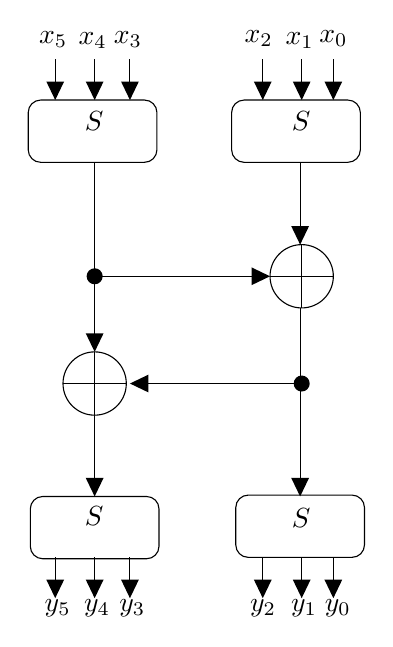
\begin{tikzpicture}[x=0.75pt,y=0.75pt,yscale=-1,xscale=1]
				%Rounded Rect [id:dp42469603179893767] 
				\draw   (280,46.67) .. controls (280,43.35) and (282.69,40.67) .. (286,40.67) -- (336,40.67) .. controls (339.31,40.67) and (342,43.35) .. (342,46.67) -- (342,64.67) .. controls (342,67.98) and (339.31,70.67) .. (336,70.67) -- (286,70.67) .. controls (282.69,70.67) and (280,67.98) .. (280,64.67) -- cycle ;
				%Rounded Rect [id:dp6966375267828862] 
				\draw   (380,237) .. controls (380,233.69) and (382.69,231) .. (386,231) -- (436,231) .. controls (439.31,231) and (442,233.69) .. (442,237) -- (442,255) .. controls (442,258.31) and (439.31,261) .. (436,261) -- (386,261) .. controls (382.69,261) and (380,258.31) .. (380,255) -- cycle ;
				%Rounded Rect [id:dp7860477123039233] 
				\draw   (281,237.67) .. controls (281,234.35) and (283.69,231.67) .. (287,231.67) -- (337,231.67) .. controls (340.31,231.67) and (343,234.35) .. (343,237.67) -- (343,255.67) .. controls (343,258.98) and (340.31,261.67) .. (337,261.67) -- (287,261.67) .. controls (283.69,261.67) and (281,258.98) .. (281,255.67) -- cycle ;
				%Rounded Rect [id:dp6309455241767805] 
				\draw   (378,46.67) .. controls (378,43.35) and (380.69,40.67) .. (384,40.67) -- (434,40.67) .. controls (437.31,40.67) and (440,43.35) .. (440,46.67) -- (440,64.67) .. controls (440,67.98) and (437.31,70.67) .. (434,70.67) -- (384,70.67) .. controls (380.69,70.67) and (378,67.98) .. (378,64.67) -- cycle ;
				%Flowchart: Or [id:dp43111622810218186] 
				\draw   (396.5,125.58) .. controls (396.5,117.16) and (403.33,110.33) .. (411.75,110.33) .. controls (420.17,110.33) and (427,117.16) .. (427,125.58) .. controls (427,134.01) and (420.17,140.83) .. (411.75,140.83) .. controls (403.33,140.83) and (396.5,134.01) .. (396.5,125.58) -- cycle ; \draw   (396.5,125.58) -- (427,125.58) ; \draw   (411.75,110.33) -- (411.75,140.83) ;
				%Flowchart: Or [id:dp07612372653447363] 
				\draw   (296.75,177.25) .. controls (296.75,168.83) and (303.58,162) .. (312,162) .. controls (320.42,162) and (327.25,168.83) .. (327.25,177.25) .. controls (327.25,185.67) and (320.42,192.5) .. (312,192.5) .. controls (303.58,192.5) and (296.75,185.67) .. (296.75,177.25) -- cycle ; \draw   (296.75,177.25) -- (327.25,177.25) ; \draw   (312,162) -- (312,192.5) ;
				%Straight Lines [id:da8522631997534107] 
				\draw    (312,70.67) -- (312,110.33) -- (312,159) ;
				\draw [shift={(312,162)}, rotate = 270] [fill={rgb, 255:red, 0; green, 0; blue, 0 }  ][line width=0.08]  [draw opacity=0] (8.93,-4.29) -- (0,0) -- (8.93,4.29) -- cycle    ;
				%Straight Lines [id:da9683498029167241] 
				\draw    (312,190) -- (312,228.67) ;
				\draw [shift={(312,231.67)}, rotate = 270] [fill={rgb, 255:red, 0; green, 0; blue, 0 }  ][line width=0.08]  [draw opacity=0] (8.93,-4.29) -- (0,0) -- (8.93,4.29) -- cycle    ;
				%Straight Lines [id:da7114989354511323] 
				\draw    (411,70.67) -- (411,107.33) ;
				\draw [shift={(411,110.33)}, rotate = 270] [fill={rgb, 255:red, 0; green, 0; blue, 0 }  ][line width=0.08]  [draw opacity=0] (8.93,-4.29) -- (0,0) -- (8.93,4.29) -- cycle    ;
				%Straight Lines [id:da028449341110133863] 
				\draw    (411,141) -- (411,228.67) ;
				\draw [shift={(411,231.67)}, rotate = 270] [fill={rgb, 255:red, 0; green, 0; blue, 0 }  ][line width=0.08]  [draw opacity=0] (8.93,-4.29) -- (0,0) -- (8.93,4.29) -- cycle    ;
				%Straight Lines [id:da37227579139782074] 
				\draw    (312,125.58) -- (393.5,125.58) ;
				\draw [shift={(396.5,125.58)}, rotate = 180] [fill={rgb, 255:red, 0; green, 0; blue, 0 }  ][line width=0.08]  [draw opacity=0] (8.93,-4.29) -- (0,0) -- (8.93,4.29) -- cycle    ;
				\draw [shift={(312,125.58)}, rotate = 0] [color={rgb, 255:red, 0; green, 0; blue, 0 }  ][fill={rgb, 255:red, 0; green, 0; blue, 0 }  ][line width=0.75]      (0, 0) circle [x radius= 3.35, y radius= 3.35]   ;
				%Straight Lines [id:da09500204271101675] 
				\draw    (411.75,177.25) -- (332,177.25) ;
				\draw [shift={(329,177.25)}, rotate = 360] [fill={rgb, 255:red, 0; green, 0; blue, 0 }  ][line width=0.08]  [draw opacity=0] (8.93,-4.29) -- (0,0) -- (8.93,4.29) -- cycle    ;
				\draw [shift={(411.75,177.25)}, rotate = 180] [color={rgb, 255:red, 0; green, 0; blue, 0 }  ][fill={rgb, 255:red, 0; green, 0; blue, 0 }  ][line width=0.75]      (0, 0) circle [x radius= 3.35, y radius= 3.35]   ;
				%Straight Lines [id:da7216603342387058] 
				\draw    (293,21) -- (293,37.67) ;
				\draw [shift={(293,40.67)}, rotate = 270] [fill={rgb, 255:red, 0; green, 0; blue, 0 }  ][line width=0.08]  [draw opacity=0] (8.93,-4.29) -- (0,0) -- (8.93,4.29) -- cycle    ;
				%Straight Lines [id:da6680400534339734] 
				\draw    (427,261) -- (427,277.67) ;
				\draw [shift={(427,280.67)}, rotate = 270] [fill={rgb, 255:red, 0; green, 0; blue, 0 }  ][line width=0.08]  [draw opacity=0] (8.93,-4.29) -- (0,0) -- (8.93,4.29) -- cycle    ;
				%Straight Lines [id:da8526371010233802] 
				\draw    (411.75,261) -- (411.75,277.67) ;
				\draw [shift={(411.75,280.67)}, rotate = 270] [fill={rgb, 255:red, 0; green, 0; blue, 0 }  ][line width=0.08]  [draw opacity=0] (8.93,-4.29) -- (0,0) -- (8.93,4.29) -- cycle    ;
				%Straight Lines [id:da6981601366843095] 
				\draw    (393,261) -- (393,277.67) ;
				\draw [shift={(393,280.67)}, rotate = 270] [fill={rgb, 255:red, 0; green, 0; blue, 0 }  ][line width=0.08]  [draw opacity=0] (8.93,-4.29) -- (0,0) -- (8.93,4.29) -- cycle    ;
				%Straight Lines [id:da5911662054724454] 
				\draw    (329,261) -- (329,277.67) ;
				\draw [shift={(329,280.67)}, rotate = 270] [fill={rgb, 255:red, 0; green, 0; blue, 0 }  ][line width=0.08]  [draw opacity=0] (8.93,-4.29) -- (0,0) -- (8.93,4.29) -- cycle    ;
				%Straight Lines [id:da3165088675709036] 
				\draw    (312,261) -- (312,277.67) ;
				\draw [shift={(312,280.67)}, rotate = 270] [fill={rgb, 255:red, 0; green, 0; blue, 0 }  ][line width=0.08]  [draw opacity=0] (8.93,-4.29) -- (0,0) -- (8.93,4.29) -- cycle    ;
				%Straight Lines [id:da34235095441645025] 
				\draw    (293,261) -- (293,277.67) ;
				\draw [shift={(293,280.67)}, rotate = 270] [fill={rgb, 255:red, 0; green, 0; blue, 0 }  ][line width=0.08]  [draw opacity=0] (8.93,-4.29) -- (0,0) -- (8.93,4.29) -- cycle    ;
				%Straight Lines [id:da9169393016789211] 
				\draw    (427,21) -- (427,37.67) ;
				\draw [shift={(427,40.67)}, rotate = 270] [fill={rgb, 255:red, 0; green, 0; blue, 0 }  ][line width=0.08]  [draw opacity=0] (8.93,-4.29) -- (0,0) -- (8.93,4.29) -- cycle    ;
				%Straight Lines [id:da7533568138302713] 
				\draw    (411.75,21) -- (411.75,37.67) ;
				\draw [shift={(411.75,40.67)}, rotate = 270] [fill={rgb, 255:red, 0; green, 0; blue, 0 }  ][line width=0.08]  [draw opacity=0] (8.93,-4.29) -- (0,0) -- (8.93,4.29) -- cycle    ;
				%Straight Lines [id:da08630039198921913] 
				\draw    (393,21) -- (393,37.67) ;
				\draw [shift={(393,40.67)}, rotate = 270] [fill={rgb, 255:red, 0; green, 0; blue, 0 }  ][line width=0.08]  [draw opacity=0] (8.93,-4.29) -- (0,0) -- (8.93,4.29) -- cycle    ;
				%Straight Lines [id:da6264691949263468] 
				\draw    (329,21) -- (329,37.67) ;
				\draw [shift={(329,40.67)}, rotate = 270] [fill={rgb, 255:red, 0; green, 0; blue, 0 }  ][line width=0.08]  [draw opacity=0] (8.93,-4.29) -- (0,0) -- (8.93,4.29) -- cycle    ;
				%Straight Lines [id:da4214884257566729] 
				\draw    (312,21) -- (312,37.67) ;
				\draw [shift={(312,40.67)}, rotate = 270] [fill={rgb, 255:red, 0; green, 0; blue, 0 }  ][line width=0.08]  [draw opacity=0] (8.93,-4.29) -- (0,0) -- (8.93,4.29) -- cycle    ;
				
				% Text Node
				\draw (405.75,236.07) node [anchor=north west][inner sep=0.75pt]    {$S$};
				% Text Node
				\draw (306,235.4) node [anchor=north west][inner sep=0.75pt]    {$S$};
				% Text Node
				\draw (405.75,45.07) node [anchor=north west][inner sep=0.75pt]    {$S$};
				% Text Node
				\draw (306,45.07) node [anchor=north west][inner sep=0.75pt]    {$S$};
				% Text Node
				\draw (284,6.4) node [anchor=north west][inner sep=0.75pt]    {$x_{5}$};
				% Text Node
				\draw (419,6.07) node [anchor=north west][inner sep=0.75pt]    {$x_{0}$};
				% Text Node
				\draw (402.75,6.73) node [anchor=north west][inner sep=0.75pt]    {$x_{1}$};
				% Text Node
				\draw (383,6.07) node [anchor=north west][inner sep=0.75pt]    {$x_{2}$};
				% Text Node
				\draw (320,6.4) node [anchor=north west][inner sep=0.75pt]    {$x_{3}$};
				% Text Node
				\draw (303,6.73) node [anchor=north west][inner sep=0.75pt]    {$x_{4}$};
				% Text Node
				\draw (286.67,280) node [anchor=north west][inner sep=0.75pt]    {$y_{5}$};
				% Text Node
				\draw (421.67,280) node [anchor=north west][inner sep=0.75pt]    {$y_{0}$};
				% Text Node
				\draw (405.42,280) node [anchor=north west][inner sep=0.75pt]    {$y_{1}$};
				% Text Node
				\draw (385.67,280) node [anchor=north west][inner sep=0.75pt]    {$y_{2}$};
				% Text Node
				\draw (322.67,280) node [anchor=north west][inner sep=0.75pt]    {$y_{3}$};
				% Text Node
				\draw (305.67,280) node [anchor=north west][inner sep=0.75pt]    {$y_{4}$};
			\end{tikzpicture}
		\end{figure}\ \\
		입력차분 $\alpha = 1(000\ 001)$에 대하여 차분확률  $P[\alpha\to\beta]$가 최대가 되는 $\beta$와 차분확률을 구하면?
	\end{enumerate}
	\begin{proof}[\sol]
		\ \begin{enumerate}[(a)]
			\item 표의 3번째 줄에 의해서 $P[\alpha\to\alpha]=P[010\to 010]=0.5$.
			\item Let $x=(x_1x_2x_3)_2$ and $S[x]=(y_3y_2y_1)_2$. Consider $a=(101)_2$ and $b=(011)_2$: \begin{figure}[h!]\centering
				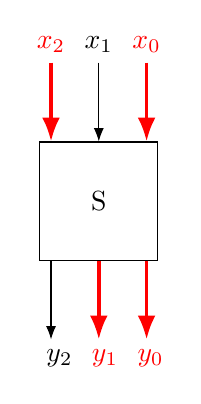
\begin{tikzpicture}[>=Latex, node distance=1cm and 0cm]
					% Nodes for inputs x
					\node (x2) {\textcolor{red}{$x_2$}};
					\node (x1) [right=of x2] {{$x_1$}};
					\node (x0) [right=of x1] {\textcolor{red}{$x_0$}};
					
					% S-Box
					\node (S) [draw, minimum size=1.5cm, below=of x1, xshift=0cm] {S};
					
					% Nodes for outputs y
					\node (y2) [below=of S, xshift=-.5cm] {$y_2$};
					\node (y1) [right=of y2] {\textcolor{red}{$y_1$}};
					\node (y0) [right=of y1] {\textcolor{red}{$y_0$}};
					
					% Arrows from x to S
					\draw[->, red, line width=1.25] (x2) -- (x2|-S.north);
					\draw[->] (x1) -- (x1|-S.north);
					\draw[->, red, line width=1.25] (x0) -- (x0|-S.north);
					
					% Arrows from S to y (ensuring alignment with x_i nodes)
					\draw[->] (S.south-|x2) -- (x2|-y2.north);
					\draw[->, red, line width=1.25] (S.south-|x1) -- (x1|-y1.north);
					\draw[->, red, line width=1.25] (S.south-|x0) -- (x0|-y0.north);
				\end{tikzpicture}
			\end{figure}\ \\	
			\begin{table}[h!]\centering\renewcommand{\arraystretch}{1.5}
				\begin{tabular}{ccc|ccc|cc}
					\toprule[1.2pt]
					\textcolor{red}{$x_2$} & {$x_1$} & \textcolor{red}{$x_0$} & $y_2$ & \textcolor{red}{$y_1$} & \textcolor{red}{$y_0$} & $a\cdot x=b\cdot y$ & \\
					\hline
					0 & 0 & 0 & 0 & 0 & 0 & $0=0$ & \textcolor{green}{\checkmark}\\
					0 & 0 & 1 & 0 & 1 & 0 & $1=1$ & \textcolor{green}{\checkmark}\\
					0 & 1 & 0 & 1 & 0 & 0 & $0=0$ & \textcolor{green}{\checkmark}\\
					0 & 1 & 1 & 1 & 1 & 0 & $1=1$ & \textcolor{green}{\checkmark}\\
					1 & 0 & 0 & 1 & 0 & 1 & $1=1$ & \textcolor{green}{\checkmark}\\
					1 & 0 & 1 & 1 & 1 & 1 & $0=0$ & \textcolor{green}{\checkmark}\\
					1 & 1 & 0 & 0 & 1 & 1 & $1=0$ & \textcolor{red}{\xmark}\\
					1 & 1 & 1 & 0 & 0 & 1 & $0=1$ & \textcolor{red}{\xmark}\\
					\bottomrule[1.2pt]
				\end{tabular}
			\end{table}\\ 따라서 집합 $NS(a,b)$의 원소의 개수는 6이다.
			\item 
		\end{enumerate}
	\end{proof}
\end{enumerate}

\newpage
\section{2023}
\begin{enumerate}[\bf 1.]
	\item[]
	\begin{figure}[h!]\centering
		\includegraphics[scale=.525]{final2023-1}
	\end{figure}
	\begin{proof}[\sol]
		\begin{enumerate}[(a)]
			\item $A=2$ and  $B=4$: \begin{center}
				\begin{tabular}{cc|cc|c}
					\toprule[1.2pt]
					$x$ & $x \oplus 010$ & $S[x]$ & $S[x\oplus 010]$ & $\Delta y$\\ \hline
					000 & 010 & 010 & 000 & 010 \\
					001 & 011 & 001 & 101 & 100 \\
					010 & 000 & 000 & 010 & 010 \\
					011 & 001 & 101 & 001 & 100 \\
					100 & 110 & 011 & 110 & 101 \\
					101 & 111 & 111 & 100 & 011 \\
					110 & 100 & 110 & 011 & 101 \\
					111 & 101 & 100 & 111 & 011 \\
					\bottomrule[1.2pt]
				\end{tabular}$\implies$ $P[\Delta x=2\to\Delta y=2]=2/8=1/4$.
			\end{center}
			\item \ \begin{table}[h!]\centering
				\begin{tabular}{ccc|ccc|cc}
					\toprule[1.2pt]
					\textcolor{red}{$[x_2]$} & \textcolor{red}{$[x_1]$} & $x_0$ & \textcolor{red}{$[y_2]$} & {$y_1$} & \textcolor{red}{$[y_0]$} & $a\cdot x=b\cdot y$ & \\
					\hline
					0 & 0 & 0 & 0 & 1 & 0 & $0=0$ & \textcolor{green}{\checkmark}\\
					0 & 0 & 1 & 0 & 0 & 1 & $0=1$ & \textcolor{red}{\xmark}\\
					0 & 1 & 0 & 0 & 0 & 0 & $1=0$ & \textcolor{red}{\xmark}\\
					0 & 1 & 1 & 1 & 0 & 1 & $1=0$ & \textcolor{red}{\xmark}\\
					1 & 0 & 0 & 0 & 1 & 1 & $1=1$ & \textcolor{green}{\checkmark}\\
					1 & 0 & 1 & 1 & 1 & 1 & $1=0$ & \textcolor{red}{\xmark}\\
					1 & 1 & 0 & 1 & 1 & 0 & $0=1$ & \textcolor{red}{\xmark}\\
					1 & 1 & 1 & 1 & 0 & 0 & $0=1$ & \textcolor{red}{\xmark}\\
					\bottomrule[1.2pt]
				\end{tabular}$\implies$ the probability is $2/8=1/4$.
			\end{table}
		\end{enumerate}
	\end{proof}
	\item[]
	\begin{figure}[h!]\centering
		\includegraphics[scale=.57]{final2023-2}
	\end{figure}
	\begin{proof}[\sol]
		\ \\ \adjustbox{scale=1, center}{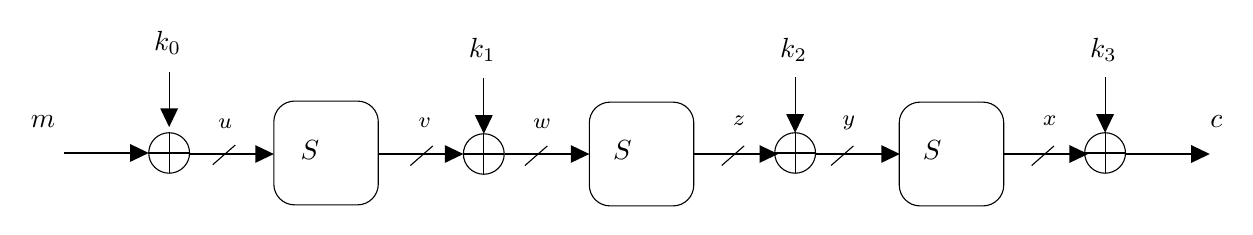
\begin{tikzpicture}[x=0.75pt,y=0.75pt,yscale=-1,xscale=1]
			%uncomment if require: \path (0,300); %set diagram left start at 0, and has height of 300	
			%Flowchart: Or [id:dp6387090213276583] 
			\draw   (114.73,150) .. controls (114.73,144.62) and (119.14,140.25) .. (124.57,140.25) .. controls (130,140.25) and (134.4,144.62) .. (134.4,150) .. controls (134.4,155.38) and (130,159.75) .. (124.57,159.75) .. controls (119.14,159.75) and (114.73,155.38) .. (114.73,150) -- cycle ; \draw   (114.73,150) -- (134.4,150) ; \draw   (124.57,140.25) -- (124.57,159.75) ;
			%Rounded Rect [id:dp2984270284803445] 
			\draw   (175,135) .. controls (175,129.48) and (179.48,125) .. (185,125) -- (215.33,125) .. controls (220.86,125) and (225.33,129.48) .. (225.33,135) -- (225.33,165) .. controls (225.33,170.52) and (220.86,175) .. (215.33,175) -- (185,175) .. controls (179.48,175) and (175,170.52) .. (175,165) -- cycle ;
			%Flowchart: Or [id:dp403217021780772] 
			\draw   (266.33,150.5) .. controls (266.33,145.12) and (270.74,140.75) .. (276.17,140.75) .. controls (281.6,140.75) and (286,145.12) .. (286,150.5) .. controls (286,155.88) and (281.6,160.25) .. (276.17,160.25) .. controls (270.74,160.25) and (266.33,155.88) .. (266.33,150.5) -- cycle ; \draw   (266.33,150.5) -- (286,150.5) ; \draw   (276.17,140.75) -- (276.17,160.25) ;
			%Rounded Rect [id:dp7969101552713898] 
			\draw   (327,135.5) .. controls (327,129.98) and (331.48,125.5) .. (337,125.5) -- (367.33,125.5) .. controls (372.86,125.5) and (377.33,129.98) .. (377.33,135.5) -- (377.33,165.5) .. controls (377.33,171.02) and (372.86,175.5) .. (367.33,175.5) -- (337,175.5) .. controls (331.48,175.5) and (327,171.02) .. (327,165.5) -- cycle ;
			%Flowchart: Or [id:dp6677888640244123] 
			\draw   (416.33,150) .. controls (416.33,144.62) and (420.74,140.25) .. (426.17,140.25) .. controls (431.6,140.25) and (436,144.62) .. (436,150) .. controls (436,155.38) and (431.6,159.75) .. (426.17,159.75) .. controls (420.74,159.75) and (416.33,155.38) .. (416.33,150) -- cycle ; \draw   (416.33,150) -- (436,150) ; \draw   (426.17,140.25) -- (426.17,159.75) ;
			%Straight Lines [id:da5362001581563707] 
			\draw    (134.4,150.5) -- (155.67,150.5) -- (172,150.5) ;
			\draw [shift={(175,150.5)}, rotate = 180] [fill={rgb, 255:red, 0; green, 0; blue, 0 }  ][line width=0.08]  [draw opacity=0] (8.93,-4.29) -- (0,0) -- (8.93,4.29) -- cycle    ;
			%Straight Lines [id:da39216223723804444] 
			\draw    (225.73,150.5) -- (247,150.5) -- (263.33,150.5) ;
			\draw [shift={(266.33,150.5)}, rotate = 180] [fill={rgb, 255:red, 0; green, 0; blue, 0 }  ][line width=0.08]  [draw opacity=0] (8.93,-4.29) -- (0,0) -- (8.93,4.29) -- cycle    ;
			%Straight Lines [id:da17543897115899898] 
			\draw    (286.4,150.5) -- (307.67,150.5) -- (324,150.5) ;
			\draw [shift={(327,150.5)}, rotate = 180] [fill={rgb, 255:red, 0; green, 0; blue, 0 }  ][line width=0.08]  [draw opacity=0] (8.93,-4.29) -- (0,0) -- (8.93,4.29) -- cycle    ;
			%Straight Lines [id:da7242342168072087] 
			\draw    (377.33,150.5) -- (398.6,150.5) -- (414.93,150.5) ;
			\draw [shift={(417.93,150.5)}, rotate = 180] [fill={rgb, 255:red, 0; green, 0; blue, 0 }  ][line width=0.08]  [draw opacity=0] (8.93,-4.29) -- (0,0) -- (8.93,4.29) -- cycle    ;
			%Straight Lines [id:da10920614678319085] 
			\draw    (436,150.5) -- (457.27,150.5) -- (473.6,150.5) ;
			\draw [shift={(476.6,150.5)}, rotate = 180] [fill={rgb, 255:red, 0; green, 0; blue, 0 }  ][line width=0.08]  [draw opacity=0] (8.93,-4.29) -- (0,0) -- (8.93,4.29) -- cycle    ;
			%Straight Lines [id:da08748396717157081] 
			\draw    (74.13,150) -- (95.4,150) -- (111.73,150) ;
			\draw [shift={(114.73,150)}, rotate = 180] [fill={rgb, 255:red, 0; green, 0; blue, 0 }  ][line width=0.08]  [draw opacity=0] (8.93,-4.29) -- (0,0) -- (8.93,4.29) -- cycle    ;
			%Straight Lines [id:da4140953307861994] 
			\draw    (124.57,110.75) -- (124.57,122.75) -- (124.57,134.5) ;
			\draw [shift={(124.57,137.5)}, rotate = 270] [fill={rgb, 255:red, 0; green, 0; blue, 0 }  ][line width=0.08]  [draw opacity=0] (8.93,-4.29) -- (0,0) -- (8.93,4.29) -- cycle    ;
			%Straight Lines [id:da4902037387269014] 
			\draw    (276.17,114) -- (276.17,126) -- (276.17,137.75) ;
			\draw [shift={(276.17,140.75)}, rotate = 270] [fill={rgb, 255:red, 0; green, 0; blue, 0 }  ][line width=0.08]  [draw opacity=0] (8.93,-4.29) -- (0,0) -- (8.93,4.29) -- cycle    ;
			%Straight Lines [id:da032438173515496604] 
			\draw    (426.17,113.5) -- (426.17,125.5) -- (426.17,137.25) ;
			\draw [shift={(426.17,140.25)}, rotate = 270] [fill={rgb, 255:red, 0; green, 0; blue, 0 }  ][line width=0.08]  [draw opacity=0] (8.93,-4.29) -- (0,0) -- (8.93,4.29) -- cycle    ;
			%Straight Lines [id:da38705791074267304] 
			\draw    (156.38,146.21) -- (145.6,155.64) ;
			%Straight Lines [id:da6577256556176674] 
			\draw    (251.58,146.61) -- (240.8,156.04) ;
			%Straight Lines [id:da9791366655045883] 
			\draw    (306.78,146.61) -- (296,156.04) ;
			%Straight Lines [id:da12965720331903818] 
			\draw    (401.58,146.61) -- (390.8,156.04) ;
			%Rounded Rect [id:dp47562690354046877] 
			\draw   (476.33,135.5) .. controls (476.33,129.98) and (480.81,125.5) .. (486.33,125.5) -- (516.67,125.5) .. controls (522.19,125.5) and (526.67,129.98) .. (526.67,135.5) -- (526.67,165.5) .. controls (526.67,171.02) and (522.19,175.5) .. (516.67,175.5) -- (486.33,175.5) .. controls (480.81,175.5) and (476.33,171.02) .. (476.33,165.5) -- cycle ;
			%Flowchart: Or [id:dp5220437140255207] 
			\draw   (565.67,150) .. controls (565.67,144.62) and (570.07,140.25) .. (575.5,140.25) .. controls (580.93,140.25) and (585.33,144.62) .. (585.33,150) .. controls (585.33,155.38) and (580.93,159.75) .. (575.5,159.75) .. controls (570.07,159.75) and (565.67,155.38) .. (565.67,150) -- cycle ; \draw   (565.67,150) -- (585.33,150) ; \draw   (575.5,140.25) -- (575.5,159.75) ;
			%Straight Lines [id:da8946446298525024] 
			\draw    (526.67,150.5) -- (547.93,150.5) -- (564.27,150.5) ;
			\draw [shift={(567.27,150.5)}, rotate = 180] [fill={rgb, 255:red, 0; green, 0; blue, 0 }  ][line width=0.08]  [draw opacity=0] (8.93,-4.29) -- (0,0) -- (8.93,4.29) -- cycle    ;
			%Straight Lines [id:da9715445749840461] 
			\draw    (585.33,150.5) -- (606.6,150.5) -- (622.93,150.5) ;
			\draw [shift={(625.93,150.5)}, rotate = 180] [fill={rgb, 255:red, 0; green, 0; blue, 0 }  ][line width=0.08]  [draw opacity=0] (8.93,-4.29) -- (0,0) -- (8.93,4.29) -- cycle    ;
			%Straight Lines [id:da12822511670510717] 
			\draw    (575.5,113.5) -- (575.5,125.5) -- (575.5,137.25) ;
			\draw [shift={(575.5,140.25)}, rotate = 270] [fill={rgb, 255:red, 0; green, 0; blue, 0 }  ][line width=0.08]  [draw opacity=0] (8.93,-4.29) -- (0,0) -- (8.93,4.29) -- cycle    ;
			%Straight Lines [id:da8312859594211475] 
			\draw    (550.91,146.61) -- (540.14,156.04) ;
			%Straight Lines [id:da06328702371456796] 
			\draw    (454.25,146.61) -- (443.47,156.04) ;
			
			% Text Node
			\draw (56.67,130.9) node [anchor=north west][inner sep=0.75pt]    {$m$};
			% Text Node
			\draw (186.67,142.9) node [anchor=north west][inner sep=0.75pt]    {$S$};
			% Text Node
			\draw (337.17,142.9) node [anchor=north west][inner sep=0.75pt]    {$S$};
			% Text Node
			\draw (116.07,89.9) node [anchor=north west][inner sep=0.75pt]    {$k_{0}$};
			% Text Node
			\draw (267.67,93.4) node [anchor=north west][inner sep=0.75pt]    {$k_{1}$};
			% Text Node
			\draw (417.67,93.4) node [anchor=north west][inner sep=0.75pt]    {$k_{2}$};
			% Text Node
			\draw (147.07,132.5) node [anchor=north west][inner sep=0.75pt]  [font=\footnotesize]  {$u$};
			% Text Node
			\draw (243.47,131.7) node [anchor=north west][inner sep=0.75pt]  [font=\footnotesize]  {$v$};
			% Text Node
			\draw (298.8,132.5) node [anchor=north west][inner sep=0.75pt]  [font=\footnotesize]  {$w$};
			% Text Node
			\draw (395.07,130.9) node [anchor=north west][inner sep=0.75pt]  [font=\footnotesize]  {$z$};
			% Text Node
			\draw (625,130.9) node [anchor=north west][inner sep=0.75pt]    {$c$};
			% Text Node
			\draw (486.5,142.9) node [anchor=north west][inner sep=0.75pt]    {$S$};
			% Text Node
			\draw (567,93.4) node [anchor=north west][inner sep=0.75pt]    {$k_{3}$};
			% Text Node
			\draw (544.4,130.9) node [anchor=north west][inner sep=0.75pt]  [font=\footnotesize]  {$x$};
			% Text Node
			\draw (447.73,130.9) node [anchor=north west][inner sep=0.75pt]  [font=\footnotesize]  {$y$};
	\end{tikzpicture}}
		Let \[\begin{array}{lclcl}
			u=m\oplus k_0 && v=S[u] && w=v\oplus k_1\\
			x=c\oplus k_3 && y=S^{-1}[x] && z=y\oplus k_2
		\end{array}\]
		\begin{enumerate}[(a)]
			\item Consider \begin{align*}
				\alpha\cdot u\oplus\beta\cdot v&=0\quad\quad\cdots\cdots\ p_1=\frac{1}{2}+\epsilon_1,\\
				\beta\cdot w\oplus\gamma\cdot z&=0\quad\quad\cdots\cdots\ p_2=\frac{1}{2}+\epsilon_2.
			\end{align*} By Piling-up Lemma, we have \begin{align*}
				\alpha\cdot u\oplus \beta\cdot(v\oplus w)\oplus\gamma\cdot z&=0\quad\quad\cdots\cdots\ p=\frac{1}{2}+2\epsilon_1\epsilon_2\\
				\alpha\cdot (m\oplus k_0)\oplus\beta\cdot k_1\oplus\gamma\cdot(S^{-1}[c\oplus k_3]\oplus k_2)&=0\\
				\alpha\cdot m\oplus\gamma\cdot S^{-1}[c\oplus k_3]&=\alpha\cdot k_0\oplus\beta\cdot k_1\oplus\gamma\cdot k_2.
			\end{align*} 여기서 확률 $p$가 최대가 되도록 $\alpha$와 $\beta$를 선택한다. 따라서 \[
			\alpha=0000\ 0001,\quad\beta=0000\ 0010,\quad\gamma=0001\ 0001.
			\]
			\item $k_3$를 찾은 경우 $y=S^{-1}[c\oplus k_3]$가 주어진다. 따라서 \begin{align*}
				a\cdot u &= b\cdot v\quad\quad\cdots\cdots\ p\\
				a\cdot(m\oplus k_0) & =b\cdot(S^{-1}[y\oplus k_2]\oplus k_1)\\
				a\cdot m\oplus b\cdot S^{-1}[y\oplus k_2]&=a\cdot k_0\oplus b\cdot k_1.
			\end{align*} 여기서 확률 $p$가 최대가 되도록 $a$와 $b$를 선택한다. 따라서 \[
			\begin{cases}
				a=0000\ 0001 \\
				b=0000\ 0011
			\end{cases}\quad\cdots\cdots p=P[a\cdot x=b\cdot S[x]]=0.5+0.4=0.9
			\]
		\end{enumerate}
	\end{proof}
	\newpage
	\item[]
	\begin{figure}[h!]\centering
		\includegraphics[scale=.5]{final2023-3}
		\includegraphics[scale=.375]{final2023-3-2}
	\end{figure}
	\begin{figure}[h!]\centering
		\includegraphics[scale=.55]{final2023-3-3}
	\end{figure}
	\begin{enumerate}[(a)]
		\item (1R) $(A,C,C,C)\xrightarrow{S}(A,C,C,C)\xrightarrow{LM}(C,A,A,A)$. Thus, \begin{center}
			(Const, Active, Active, Active)
		\end{center}
		\item (2R) $(C,A,A,A)\xrightarrow{S}(C,A,A,A)\xrightarrow{LM}(B,B,B,B)$. Thus, \begin{center}
			(Balanced, Balanced, Balanced, Balanced)
		\end{center}
		\item Blanced를 만족할 확률은 $1/2^8$이며, $2^8\times 1/2^8=1$이다. 따라서 $2^8=256$개만 하면 wrong key가 나올 수 있으니, $(P,C)$ 쌍 $2^8\times 2$ 개 정도 필요하다. Sbox 하나 당 \[
		2^8\times 2^8(\text{키후보})\times 2.
		\]
		\item 2라운드 0번째 바이트가 Balanced 인 것을 확인한다. \[
		rk_3'[0], rk_4[1], rk_4[2], rk_4[3]
		\]를 예측한다. 이는 $2^{32}$ 계산량으로 round key를 예측하는 것이므로 32 비트 ($2^{32}$) 키에 대한 전수보다 비효율적이다.
	\end{enumerate}
	\item[]
	\begin{figure}[h!]\centering
		\includegraphics[scale=.6]{final2023-4}
		\includegraphics[scale=.6]{final2023-4-2}
	\end{figure}
	\newpage
	\begin{proof}[\sol]
		\ \begin{enumerate}[(a)]
			\item $P_1=\texttt{0x00\ 00\ 00\ 00}$, $P_2=\texttt{0x00\ 00\ 01\ 00}$
			\item Consider \begin{align*}
				(\alpha, 0, 0, 0)&\xrightarrow{S\ \text{with}\ p_1}(\beta,0,0,0)\quad\quad\cdots\cdots\ \text{Round 1}\\
				&\xrightarrow{LM}(0,\beta,\beta,\beta) \\ \\
				(0,\beta,\beta,\beta)&\xrightarrow{S\ \text{with}\ p_2^3}(0,\gamma,\gamma,\gamma)\quad\quad\cdots\cdots\ \text{Round 2}\\
				&\xrightarrow{LM}(\gamma,0,0,0)\\ \\
				(\gamma,0,0,0)&\xrightarrow{S\ \text{with}\ p_3^1}(\delta,0,0,0)\quad\quad\cdots\cdots\ \text{Round 3}\\
				&\xrightarrow{LM}(0,\delta,\delta,\delta)
			\end{align*} Consider \begin{align*}
				p_1=P[\texttt{0x01}\to\texttt{0x03}]&=0.25,\\
				p_2=P[\texttt{0x03}\to\texttt{0x0F}]&=0.25,\\
				p_3=P[\texttt{0x0F}\to\texttt{0x10}]&=0.125.
		\end{align*} Then $p=\displaystyle\left(\frac{1}{4}\right)\left(\frac{1}{4}\right)^3\left(\frac{1}{8}\right)=\frac{1}{2^{11}}>\frac{1}{2^{32}}$ and \begin{align*}
		(\texttt{0x01},\texttt{0x00},\texttt{0x00},\texttt{0x00})&\xrightarrow{1R}(\texttt{0x00},\texttt{0x03},\texttt{0x03},\texttt{0x03})\quad\quad\cdots\cdots\ p_1=1/4\\
		&\xrightarrow{2R}(\texttt{0x0F},\texttt{0x00},\texttt{0x00},\texttt{0x00})\quad\quad\cdots\cdots\ p_2^3=1/4^3\\
		&\xrightarrow{3R}(\texttt{0x00},\texttt{0x10},\texttt{0x10},\texttt{0x10})\quad\quad\cdots\cdots\ p_3=1/8.
	\end{align*}
		\end{enumerate}
	\end{proof}
	\newpage
	\item[]
	\begin{figure}[h!]\centering
	\includegraphics[scale=.45]{final2023-5}
	\includegraphics[scale=.55]{final2023-5-2}
	\end{figure}	
	\begin{figure}[h!]\centering
		\includegraphics[scale=.55]{final2023-5-3}
	\end{figure}\
	\begin{proof}[\sol]
		\ \begin{enumerate}[(a)]
			\item 입력 차분 $(0,\alpha)$, 5라운드 차분 $(\alpha,0)$. 5R 불능차분특성: \[
			\alpha\oplus\alpha=0=\gamma\neq 0.
			\]
			\item Consider $\Delta P=P_1\oplus P_2=(0,14\oplus 13)=(0,3)$. Then\begin{itemize}
				\item $CL_1\oplus CL_2=7\oplus 4=3=\alpha$;
				\item $CR_1\oplus CR_2=F(CL_1,k_6)\oplus F(CL_2,k_6)$을 만족하는 $k_6$는 키 후보에서 삭제.
				\begin{itemize}
					\item $CR_1\oplus CR_2=15\oplus 3=2$
					\item \ \\ \adjustbox{scale=.9, center}{\begin{tabular}{c|cc|cc|c}
						$k_6$ & $0111\oplus k_6$ & $0100\oplus k_6$ & $S[0111\oplus k_6]$ & $S[0100\oplus k_6]$ & $\Delta=S[CL_1\oplus k_6]\oplus S[CL_2\oplus k_6]$ \\ \hline\hline
						$\vdots$ & $\vdots$ & $\vdots$ & $\vdots$ & $\vdots$ & $\vdots$ \\ \hline
						0100 & 0011 & 0000 & 0010 & 0000 & 0010
					\end{tabular}}
				\end{itemize}
			\end{itemize}\ \\ Thus, $k\neq 0100$
		\end{enumerate}
	\end{proof}
	\newpage
	\item[]
	\begin{figure}[h!]\centering
		\includegraphics[scale=.55]{final2023-6}
	\end{figure}
	\begin{proof}[\sol]
		Note that \[
		\displaystyle 1-\left(1-\frac{ECR\cdot mt}{2^{64}}\right)^{\ell}.
		\] Since $(1-a)^b=\exp(-ab)$ ($\lim\limits_{h\to 0}(1+h)^{1/h}=e$, $\lim\limits_{a\to 0}(1-a)^b=\lim\limits_{a\to 0}[(1-a)^{-1/a}]^{-ab}=\exp(-ab)$), we have \[
		1-\exp(-\frac{ECR\cdot mt\ell}{2^{64}})=1-\exp(-0.8).
		\]
	\end{proof}
\end{enumerate}

\footer{Department of Information Security, Cryptology and Mathematics\\
	College of Science and Technology\\
	Kookmin University}

\newpage
%\begin{thebibliography}{99}
	
\bibitem{youtube_MariaEichlseder}
``Cryptanalysis - L6 Differential Cryptanalysis'' YouTube, uploaded by 
Maria Eichlseder, 22 April 2021, \url{https://www.youtube.com/watch?v=GQX8W8zKf2Q}

\bibitem{youtube_JacksonInfoSec}
``The Differential Distribution Table (DDT) of a S-Box'' YouTube, uploaded by 
JacksonInfoSec, 5 August 2021, \url{https://www.youtube.com/watch?v=di90_oL4lxk}

	
\end{thebibliography}
%\bibliography{category-theory-note-ref}
%\bibliographystyle{abbrv}
\end{document}